\documentclass{article}
\usepackage{lmodern}
\usepackage[utf8]{inputenc}
%\usepackage[spanish, activeacute]{babel}
\usepackage{mathtools}
\usepackage{amsthm}
\usepackage{amssymb}
\usepackage{tikz}
\usepackage{xcolor}
\usepackage{enumitem}
\usepackage{ragged2e}
\renewcommand{\proofname}{Dem:}

\begin{document}

	%Ejercico 1.
	\begin{justify}
		1. ¿Será posible cubrir un tablero de ajedrez al cual se la han quitado dos esquinas opuestas utilizando fichas de dominó? 
		Suponiendo que cada ficha cubre horizontalmente
		dos casillas del tablero.
	\end{justify}
	Sea $G$ una gráfica asociado al tablero de ajedrez, donde : \\
	\begin{enumerate}
	\item Cada casilla es un vertice
	\item Dos vertices son adyacentes su las casiilas comparten lado
	\end{enumerate}	

	Coloreando el tablero alternamente de blanco y negro obtenemos una bipartición. \\
	\begin{center}
	$\Rightarrow   V(G) = B U N$ \\
	\end{center}
	Cada ficha de domino cubre exactamente dos casillas adyacentes, una blanca y una negra. Por lo tanto, el tablero con fichas de dominó
	equivale a encontrar un emparejamiento perfecto en $G$. \\
	El tablero original tiene : \\
	\begin{center}
	$|B| = 32 = |N|$ \\
	\end{center}
	Sin embargo, las esquinas opuestas tienen el mismo color. Al removerlas, una de las partes de la bipartición pierde dos vertices entonces
	.S.p,g dicidimos quitar blancas y nos queda: \\
	\begin{center}
	$|B| = 30 \wedge |N| = 32$ \\
	\end{center}
	Pero un emparejamiento perfecto en una gráfica bipartita debe emparejar todos los vertices de un lado con vertices del otro lado, por lo que
	ambas partes deben tener la misma cardinalidad. \\
 	\newline Como esto no ocurre la gráfica no puede tener un emparejamiento perfecto. \\
	$\therefore$ No es posible cubrir el tablero quitando dos esquinas opuestas. \\
	\newpage
	%Ejercicio 2.
	\begin{justify}
	2. Demuestra que un árbol tiene a lo más un emparejamiento perfecto.
	\end{justify}
	\begin{proof} Contradicción. \\
	Sea $T$ un árbol y supongamos que tiene dos emparejamientos perfectos distintos. $M_1 , M_2$\\
	Como son distintos existe una arista t.q. \\
	\begin{center}
	$e_1 \in M_1 \ M_2 $
	\end{center}
	Sea $v_1$ un extremo de $e_1$ y $v_2$ el otro. Como $M_2$ es perfecto, $v_2$ debe de estar emparejado mediante una arista, entonces. 
	\begin{center}
	$e_2 \in M_2$
	\end{center}
	Ademas $e_2 \neq e_1$ puesto que $e_1 \notin M_2$ \\
	Sea $v_3$ el otro extremo de $e_2$. Como $M_1$ es perfecto, $v_3$ tiene que estar emparejado mediante una arista, entonces. \\
	\begin{center}
	$e_3 \in M_1$ \\
	Con $e_3 \neq e_2$
	\end{center} 

	Repitiendo este proceso obtenemos una sucesión de aristas alternas entre $M_1$ y $M_2$ 
	\newline
	Como la gráfica tiene un número finito de vertices, eventualmente algún vertice se repite, formando un ciclo, pero contradice que $T$ sea un
	arbol ya que estos son acíclicos. \\
	$T$ no puede tener dos emparejamientos perfectos distintos\\
	$\therefore$  Un árbol tiene a lo más un emparejamiento perfecto. 
	
	\end{proof}
	\begin{justify}
	3. Sea $G$ una gráfica trazable. Demuestra que $G$ tiene un emparejamiento perfecto.
	\end{justify}
	\begin{proof}
	Propongamos un contraejemplo. Para ver que es falso en general. \\
	Consideremos la gráfica $P_3$. 
	\begin{center}
		$P_3 = (v_1,v_2,v_3)$
	\end{center}
	Y claramente se ve que es una gráfica trazable, pues la trayectoria $(v_1,v_2,v_3)$ pasa por todos los vertices exactamente una vez, $i.e$ es una
	trayectoria hamiltoniana. 
	\newline Ahora veamos sus emparejamientos. Los caminos aristas $P_3$ son: \\
	\begin{center}
		$v_1v_2 , v_2v_3$
	 \end{center}
	Cualquier emparejamiento puede contener a lo más una de estás aristas, ya que ambas inciden en el vértice $v_2$ \\
	Por lo tanto, cualquier emparejamiento deja necesariamente un vertice sin emparejar.
	\newline Así, $P_3$ no tiene emparejamiento perfecto. \\
	Concluimos que existe una gráfica trazable que no tiene emparejamiento perfecto.



	\end{proof}
\newpage
	%Ejercicio 4.
	\begin{justify}
	4. Determina cuántos emparejamientos perfectos tiene $k_6$.  \\	
	Necesitamos encontrar un conjunto $M \subseteq E(K_6) $ donde las aristas no compartan ningún vértice \textbf{(Def 1 )}   y además que todos los vertices de $k_6$ 
	tengan algún emparejamiento. \\   	
	Tenemos la siguiente gráfica $k_6$ Y tomamos un vértice arbitrario. En esta caso $v_1$ \\
	
	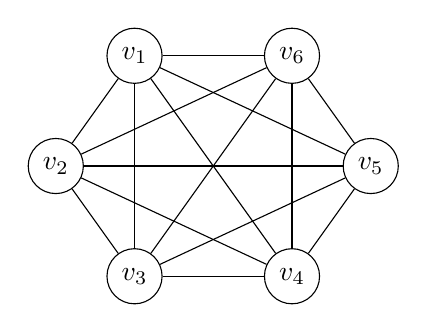
\begin{tikzpicture}[
			 vertice/.style={circle, draw, minimum size=0.7cm, inner sep=0pt}
  		]
	

	%Creamos los vertices

		\node[vertice] (v1) at (-1, 1.4) {$v_1$};
 		\node[vertice](v2) at (-2,0){$v_2$};
		\node[vertice](v3) at (-1,-1.4){$v_3$};
		\node[vertice](v4) at (1,-1.4){$v_4$};
		\node[vertice](v5) at (2,0){$v_5$};
		\node[vertice](v6) at (1,1.4){$v_6$};
	%Aristas v1 con las demás
		\draw (v1) -- (v2);
		\draw (v1) -- (v3);
		\draw (v1) -- (v4);
		\draw (v1) -- (v5);
		\draw (v1) -- (v6);
	%Aristas v2 con las demás
		\draw (v2) -- (v3);
		\draw (v2) -- (v4);
		\draw (v2) -- (v5);
		\draw (v2) -- (v6);
	%Aristas v3 con las demás
		\draw (v3) -- (v4);
		\draw (v3) -- (v5);
		\draw (v3) -- (v6);
	%Aristas v4 con las demás
		\draw (v4) -- (v5);
		\draw (v4) -- (v6);
	%Arstia v5 -- v6
	\draw(v5) -- (v6);	



	\end{tikzpicture}
	Nos fijamos en las aristas y vemos que tiene \underline{5 opc.} Nos agarramos un emparejamiento, digamos $v_2$ y trazamos el emparejamiento \\
	(Bloqueamos los caminos donde ya no se pueden hacer emparejamientos) \\
	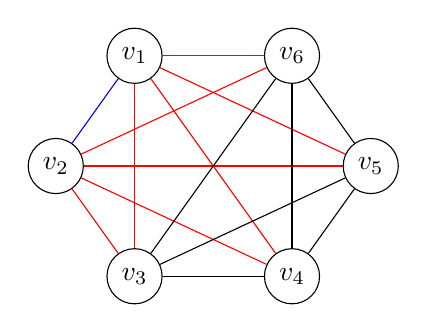
\begin{tikzpicture}[
			 vertice/.style={circle, draw, minimum size=0.7cm, inner sep=0pt}
  		]
	

	%Creamos los vertices

		\node[vertice] (v1) at (-1, 1.4) {$v_1$};
 		\node[vertice](v2) at (-2,0){$v_2$};
		\node[vertice](v3) at (-1,-1.4){$v_3$};
		\node[vertice](v4) at (1,-1.4){$v_4$};
		\node[vertice](v5) at (2,0){$v_5$};
		\node[vertice](v6) at (1,1.4){$v_6$};
	%Aristas v1 con las demás
		\draw[blue] (v1) -- (v2);
		\draw [red](v1) -- (v3);
		\draw [red](v1) -- (v4);
		\draw [red](v1) -- (v5);
		\draw [red](v1) -- (v6);
	%Aristas v2 con las demás
		\draw [red](v2) -- (v3);
		\draw [red](v2) -- (v4);
		\draw [red](v2) -- (v5);
		\draw [red](v2) -- (v6);
	%Aristas v3 con las demás
		\draw (v3) -- (v4);
		\draw (v3) -- (v5);
		\draw (v3) -- (v6);
	%Aristas v4 con las demás
		\draw (v4) -- (v5);
		\draw (v4) -- (v6);
	%Arstia v5 -- v6
	\draw(v5) -- (v6);	
	\end{tikzpicture}
	Nos paramos en el siguiente vértice en este caso $v_3$ Y nos fijamos que tiene \underline{3 opc} diferentes. Y volvemos a seleccionar un emparejamiento \\
	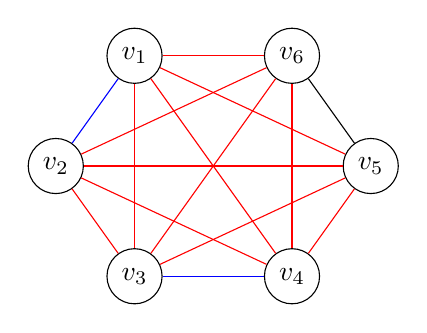
\begin{tikzpicture}[
			 vertice/.style={circle, draw, minimum size=0.7cm, inner sep=0pt}
  		]
	

	%Creamos los vertices

		\node[vertice] (v1) at (-1, 1.4) {$v_1$};
 		\node[vertice](v2) at (-2,0){$v_2$};
		\node[vertice](v3) at (-1,-1.4){$v_3$};
		\node[vertice](v4) at (1,-1.4){$v_4$};
		\node[vertice](v5) at (2,0){$v_5$};
		\node[vertice](v6) at (1,1.4){$v_6$};
	%Aristas v1 con las demás
		\draw[blue] (v1) -- (v2);
		\draw [red](v1) -- (v3);
		\draw [red](v1) -- (v4);
		\draw [red](v1) -- (v5);
		\draw [red](v1) -- (v6);
	%Aristas v2 con las demás
		\draw [red](v2) -- (v3);
		\draw [red](v2) -- (v4);
		\draw [red](v2) -- (v5);
		\draw [red](v2) -- (v6);
	%Aristas v3 con las demás
		\draw [blue](v3) -- (v4);
		\draw [red](v3) -- (v5);
		\draw [red](v3) -- (v6);
	%Aristas v4 con las demás
		\draw [red](v4) -- (v5);
		\draw [red](v4) -- (v6);
	%Arstia v5 -- v6
	\draw(v5) -- (v6);	
	\end{tikzpicture}
	\\Y al final se puede observar que queda \underline{1 opc.} disponible, en este caso $v_5$ con $v_6$.\\
	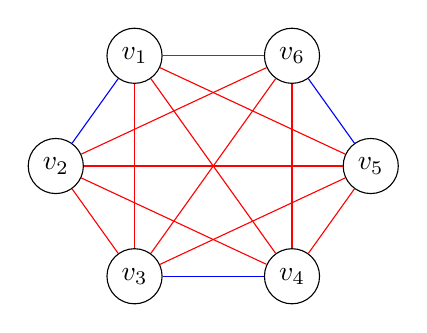
\begin{tikzpicture}[
			 vertice/.style={circle, draw, minimum size=0.7cm, inner sep=0pt}
  		]
	

	%Creamos los vertices

		\node[vertice] (v1) at (-1, 1.4) {$v_1$};
 		\node[vertice](v2) at (-2,0){$v_2$};
		\node[vertice](v3) at (-1,-1.4){$v_3$};
		\node[vertice](v4) at (1,-1.4){$v_4$};
		\node[vertice](v5) at (2,0){$v_5$};
		\node[vertice](v6) at (1,1.4){$v_6$};
	%Aristas v1 con las demás
		\draw[blue] (v1) -- (v2);
		\draw [red](v1) -- (v3);
		\draw [red](v1) -- (v4);
		\draw [red](v1) -- (v5);
		\draw [red](v1) -- (v6);
	%Aristas v2 con las demás
		\draw [red](v2) -- (v3);
		\draw [red](v2) -- (v4);
		\draw [red](v2) -- (v5);
		\draw [red](v2) -- (v6);
	%Aristas v3 con las demás
		\draw [blue](v3) -- (v4);
		\draw [red](v3) -- (v5);
		\draw [red](v3) -- (v6);
	%Aristas v4 con las demás
		\draw [red](v4) -- (v5);
		\draw [red](v4) -- (v6);
	%Arstia v5 -- v6
	\draw[blue](v5) -- (v6);	
	\end{tikzpicture}
\end{justify}
	 Con eso fomaríamos un emparejamiento perfecto en $k_6$.  \\ Note que al ser una gráfica completa se repite esta mismo secuencia. $i.e$ para cada vértice inicial
	que elijamos, primero van a ver $5 opc$, despues $3 opc$ y finalmente solo va a quedar $1 opc$. Aplicando el principio multiplicativo nos queda que. \\
					$ 5 x 3 x 1 = 15$ \\
	$\therefore$ existen 15 formas de hacer un emparejamiento perfecto en $k_6$. 
%Ejercicio 5.
\begin{justify}
	5.Encuentra un emparejamiento perfecto de la siguiente gráfica. j
ijoi
\end{justify}

\end{document}
